\documentclass[12pt]{article}
\usepackage{design_ASC}
\hypersetup{
    colorlinks=true,
    linkcolor=cyan,
    filecolor=magenta,
    urlcolor=blue,}

% Subfigures
\usepackage{subfig}

\setlength\parindent{0pt} %% Do not touch this

%% -----------------------------
%% TITLE
%% -----------------------------
\title{Exercise List \#6} %% Assignment Title

\author{Victor F. Ferrari - RA 187890\\ %% Student name
vferrari@mpc.com.br\\
MO814A/MC937A - Topics in Computer Graphics\\ %% Code and course name
\textsc{Universidade Estadual de Campinas}
}

\date{\today} %% Change "\today" by another date manually
%% -----------------------------
%% -----------------------------

%% %%%%%%%%%%%%%%%%%%%%%%%%%
\begin{document}
\setlength{\droptitle}{-5em}    
%% %%%%%%%%%%%%%%%%%%%%%%%%%
\maketitle

% --------------------------
% Start here
% --------------------------

%%%%%%%%%%%%%%%
\section{Short Answer Questions}
%%%%%%%%%%%%%%%

\subsection*{Question 1}
{\bfseries Animation techniques. You are working on a scene in a movie that will incorporate ray traced CG characters of a Vice President shooting (with buckshot) an apologetic lawyer in slow motion. (Buckshot is a type of “bullet” that consists of many small pellets that spread out as they fly through the air.) Describe what part of the animation each of the following techniques could be used for.}
\begin{itemize}
    \item \textbf{Keyframe}
    
    The keyframes would be used to mark the start and end of this sequence, starting with the VP aiming at the other person, and ending with the lawyer dead on the floor. This gives this action more creative freedom for the moment of impact.
    
    \item \textbf{Particle Systems}
    
    A good application of particle systems is the buckshot pellets. Each pellet would be a particle, and the physics of them can be simulated in slow motion, if needed.
    
    \item \textbf{Motion Capture}
    
    Motion capture could be used completely for the parts before and after the scene, and during the scene for the characters' motion, such as the lawyer going backwards with the impact, and facial expressions, if the "footage" could be customized.
\end{itemize}

\subsection*{Question 2}
{\bfseries QuadTree: The tree below represents a quadtree subdivision of a square. The left most branch is the upper left quarter, the next branch is the upper right, the third branch is the lower left, and the right most branch is the bottom left of a region. The leaf nodes are labeled A-J. Subdivide the square below to indicate the subdivision of the quad tree. Label each portion of the square with the appropriate label from the tree.}

\begin{figure}
    \centering
    \subfloat[Tree]{
    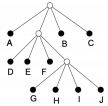
\includegraphics[width=0.35\textwidth]{images/quadtree.png}
    }
    \subfloat[Planar Subdivision]{
    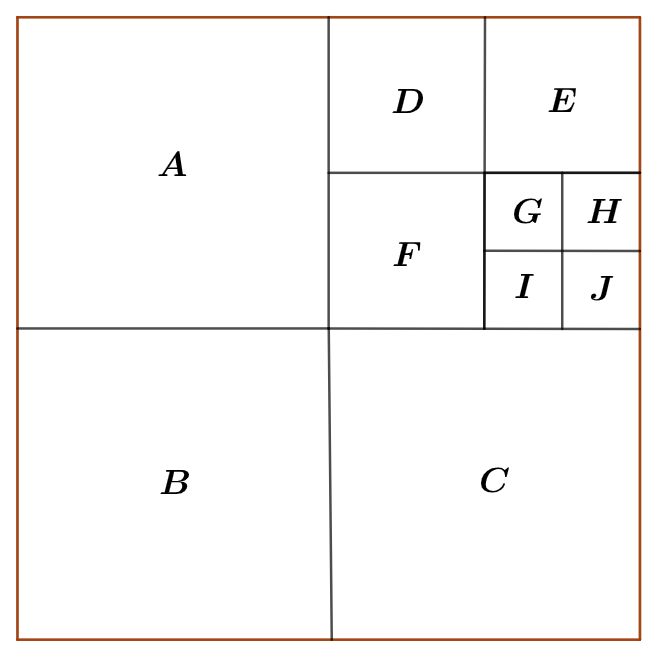
\includegraphics[width=0.35\textwidth]{images/planar_subdivision.png}
    }
    \caption{Quadtree}
    \label{fig:quad}
\end{figure}

\subsection*{Question 3}
{\bfseries Bounding boxes are one method of increasing the speed of a ray tracer. Typically, the bounding boxes are aligned with the coordinate axes. 1. Discuss the benefits/costs of axis aligned bounding boxes vs bounding boxes that are not axis aligned. 2. Discuss the benefits/costs of using bounding spheres instead of bounding boxes.}

Axis-aligned bounding boxes are used often because they give a moderately tight fit for the object, while still being fast to compute with. The problem with this approach is the need to update in every rotation, so it is not a fixed box, it has to be managed. In contrast, unaligned bounding boxes do not have this problem, but to do that they have to encompass all possible rotations of the object. This makes so that the fit is not as tight as the AABB, having to encompass a bounding sphere.

Bounding spheres are better than unaligned bounding boxes because they have the same advantages, while giving the best fit for a rotationally invariant bounding volume. But, while it can give a better fit than the unaligned bounding box, it still does not guarantee a very tight fit, so the AABB can be a better solution if updating after every rotation is feasible.

\subsection*{Question 4}
{\bfseries Ray Tracing Techniques. There are a large number of techniques for improving the realism of ray traced images. Briefly describe how each of the techniques below modifies the lighting calculation: 1) Texture Mapping, 2) Bump Mapping, 3) Displacement Mapping. Which of these techniques would be most appropriate for modeling each of the following?}
\begin{itemize}
    \item \textbf{A picture hung on a wall}: Texture Mapping
    \item \textbf{A marble statue}: Texture Mapping if the geometry already has all the detail in the statue. An optimization would be to use a more simple geometry, and use bump mapping for some of the details.
    \item \textbf{A golf ball (with no logo)}: Bump Mapping
    \item \textbf{A patterned tile floor}: Bump Mapping, but texture mapping could be used if the details between the tiles are in the geometry.
    \item \textbf{The ripples created by dropping a stone in a pool of water}: Displacement Mapping
    \item \textbf{A wooden table top}: Bump Mapping if the surface is smooth, but displacement mapping could be a good solution if the wood is too irregular.
\end{itemize}

Texture mapping does not affect lighting at all, being a flat 2D image mapped to an object affecting color. A similar answer can be said for Bump Mapping, since it does not alter the geometry of the object, only giving the appearance of complicated geometry. Displacement mapping, on the other hand, affects lighting directly, because the geometry is being altered, and therefore the new geometry will have different interactions with light, especially when using ray tracing.

\subsection*{Question 5}
{\bfseries Aliasing. Name and describe two objectionable visual artifacts that are caused by aliasing.}

Aliasing can cause edges to seem "jagged", similar to "stairs" instead of a line. It can also lead to false texture patterns. This can be seen on a static image, but in moving images strobing or flickering can be present as well.

\subsection*{Question 6}
{\bfseries Animation. What are “key frames” and “in between frames” in computer assisted key frame animation?}

Key frames in a motion scene are frames that mark the beginning and end of a transition, such as a gesture, motion, etc. These usually are the most important frames in the motion. The in between frames are the ones that represent the motion, the transition itself between a key frame and another.

\subsection*{Question 7}
{\bfseries Hidden Surface Removal. The Painter’s algorithm for hidden surface removal is not an on-line algorithm, but z-buffering is. What do we mean by an on-line algorithm for hidden surface removal?.}

In the Painter's Algorithm, all polygons are drawn once, including the hidden ones. It's not an algorithm to skip drawing those polygons, but one to not display them, and draw others on top of them. Meanwhile, the z-buffer algorithm detects hidden surfaces, and only draws the ones on top. So an online algorithm means that it actively decides what to draw before drawing.

\subsection*{Question 8}
{\bfseries Animation. If you had to make a commercial tomorrow that included a running human, how would you animate the motion of the human?}

The process would start by modeling the human as a mesh. With the model, the animation process starts by making keyframes representing a step. So there is a keyframe for each step that is both the end of the step and the beginning of the next. The keyframes represent contact, so the model would be slightly squashed.

Then, in the inbetween frames, since we are representing motion, the human could be slightly stretched to convey that information better. The properties of the activity would have to be calculated (weight, speed, size, etc), and based on that the timing of the animation (amount of inbetweens) would be set. Some attention has to go to the first few frames before and after each keyframe, since it marks the transition between one action and the next. Other keyframes might be needed, depending on the realism objective.

Another important aspect is the difference in movement in different parts of the body in each part of a step. The movement starts at the hip and leg, and the arm movements are usually synchronized. Some other details could be accounted for (amount of other actions on screen, facial expressions), but the answer so far is the main process.

\subsection*{Question 9}
{\bfseries Rendering. A major rendering technique was invented by thinking how sunlight shines through a window and bounces around to illuminate the walls, ceiling, and floor of a room. Name that technique.}

This lighting technique is a global illumination method called \textbf{ray tracing}. Specifically, the variation called \textbf{light tracing}, since the rays are traced from the light source, instead of from the viewer.

\subsection*{Question 10}
{\bfseries Shaders. Is the following code a vertex shader or a fragment shader?
\begin{verbatim}
void main(void) { glFragColor = glFrontColor; }    
\end{verbatim}
}

This code is a fragment shader, applying to a fragment the color that is passed through the vertex shader.

\end{document}